\section{Current usage of actor systems}
\begin{frame}[fragile]
\frametitle{in Distributed systems}
\begin{tikzpicture}[remember picture,overlay]
    \node[xshift=-3cm,yshift=-2cm] at (current page.north east) {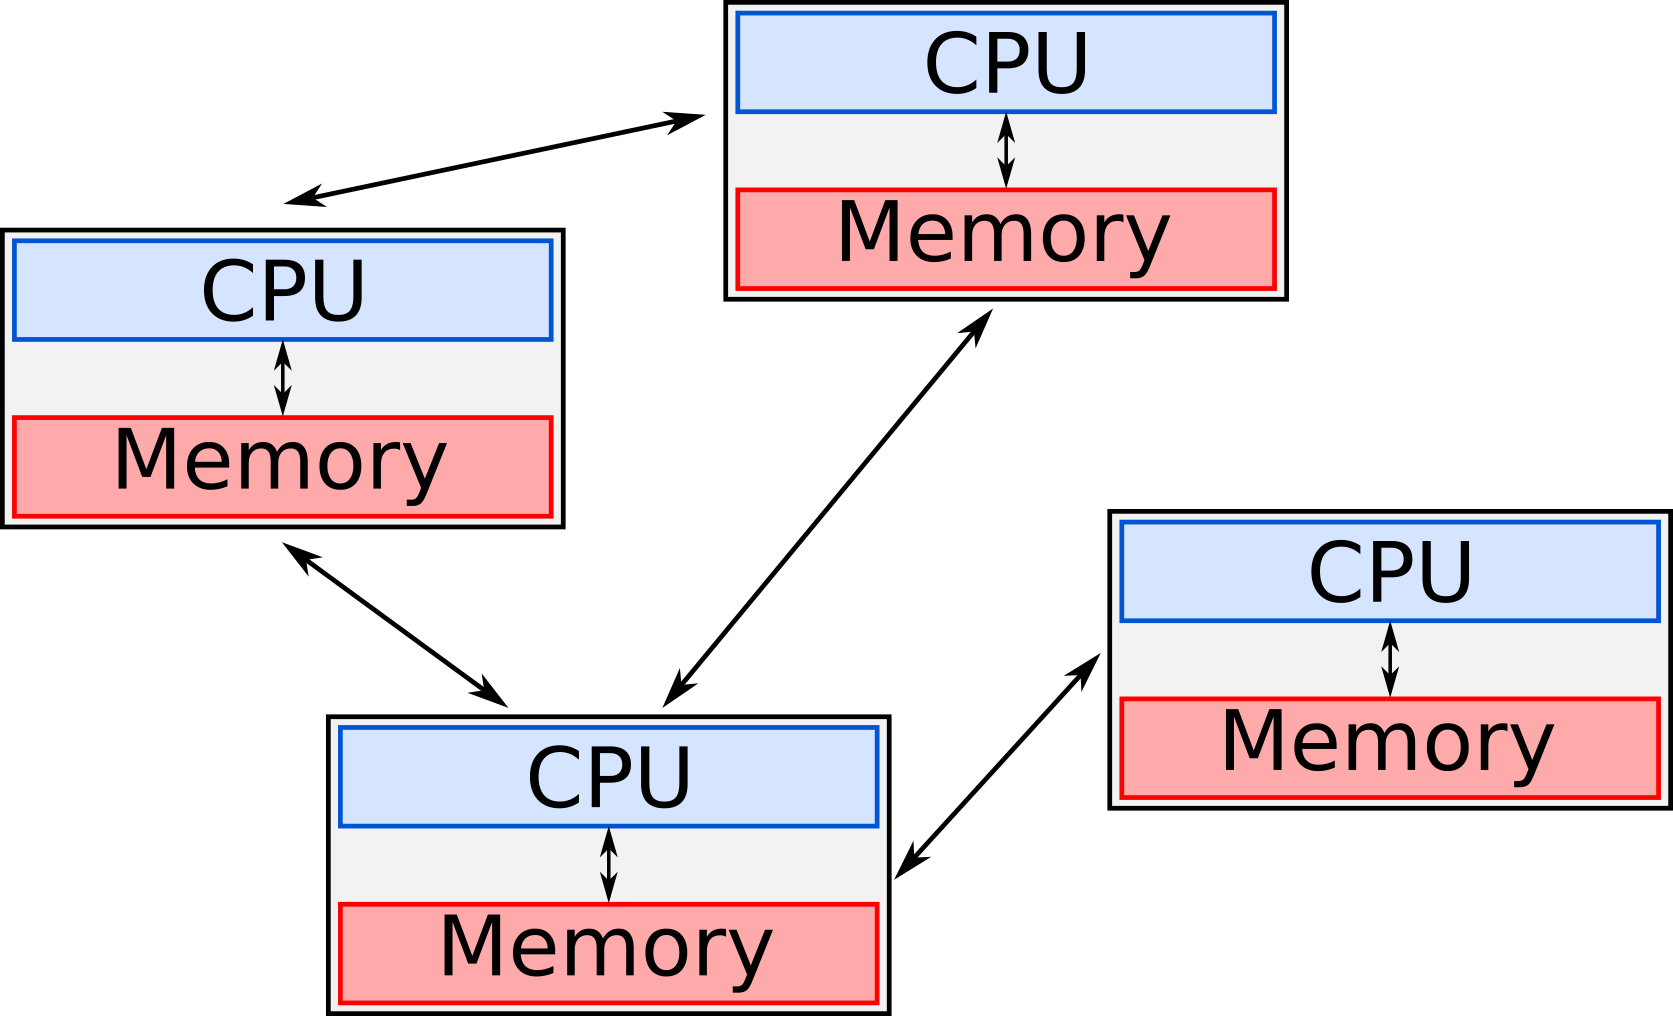
\includegraphics[width=5cm]{distr.png}};
\end{tikzpicture}
\begin{itemize}
\item Naive: map actors directly to clients
\item More suitable: map actors to program parts, e.g. individual services, users, etc
\textrightarrow e.g. {\it Facebook} chat, {\it Twitter} queues, {\it Halo 4} services, {\it Lift} web-app framework
\item HPC: actor model highly scalable (with care), e.g. ActorX10 project at TUM
\item Microservices: composition of independent services
\end{itemize}
\end{frame}

\begin{frame}
\frametitle{in Embedded systems}
\begin{itemize}
\item in system level design: model components of the system as actors \textrightarrow model-based design (capture requirements of ES) \textrightarrow enables better abstraction, definition of interface, reasoning over execution
\item on application level: e.g. ActorX10 project, model stages of algorithm as actors, pipeline execution to achieve high utilization \textrightarrow optimization of stages possible
\end{itemize}
\end{frame}